%% PREAMBLE
\documentclass[12pt]{article}

\usepackage[utf8]{inputenc}
\usepackage[margin=1in]{geometry}
\usepackage{amsmath}
\usepackage{tabularx}
\usepackage{booktabs}
\usepackage{caption}
\usepackage{graphicx}
\usepackage{float}
\usepackage{parskip}
\usepackage{dcolumn}
\usepackage{longtable}
\usepackage{xcolor}
\usepackage{hyperref}
\usepackage[backend=biber,style=apa,natbib]{biblatex}
\addbibresource{bib.bib}

\hypersetup{colorlinks=true, linkcolor=black, urlcolor=blue, citecolor=black}

%% FRONT MATTER
\title{The Broad Center Superintendent Research Dataset:\\U.S.\ Public School Superintendents, 2025--2026}
\date{April 2026}

\begin{document}

\maketitle

\section{Overview}

This document summarizes the U.S. School District Superintendents dataset for the 2025--2026 school year. The dataset identifies the superintendent (or equivalent top administrator) for every regular public school district in the United States.

The underlying data are in \textbf{\texttt{superintendents\_2025-2026\_processed.xlsx}}. Figures and tables are produced by \textbf{\texttt{descriptive\_stats.R}} and can be found in \textbf{\texttt{output/figures/}}. See \textbf{\texttt{super\_api\_README.md}} for full documentation.

This project uses agentic AI with web search. The vast majority of school districts publish their superintendent's name on their official website or in state education department records, making systematic web-based identification both feasible and accurate. Web sources include official district and state department of education websites, local news articles, and Facebook posts. Each district's superintendent was identified using a four-model AI pipeline that searched official district and state websites, extracted structured information, and independently verified results across models from different providers---reducing the risk of correlated errors:
\begin{itemize}
    \item Perplexity Sonar Pro Search
    \item OpenAI GPT-4.1 Mini
    \item Google Gemini 2.5 Pro
    \item Anthropic Claude Sonnet 4.5
\end{itemize}
Manual testing across iterative benchmark samples suggests that records are at least 95\% accurate.

The dataset covers \textbf{13,195 school districts} across all 50 states, the District of Columbia, and U.S.\ territories.

\subsection{Intended Uses}

The dataset is designed for research on school district leadership, superintendent labor markets, and educational governance. Primary applications include cross-sectional studies of superintendent characteristics and their relationship to student outcomes, analysis of leadership gender gaps, and as a baseline roster for tracking year-to-year turnover. The data can be linked to student achievement, finance, and demographic files using \texttt{LEAID}, the seven-digit NCES local education agency identifier (zero-padded), which links directly to the CCD \citep{nces_ccd}, EDFacts, and the Stanford Education Data Archive. Bureau of Indian Education districts and charter schools are excluded from this dataset but are present in the CCD; unmatched LEAIDs in a merge typically reflect these exclusions.

\subsection{Relationship to Prior Data}

This dataset extends and complements the existing Broad Center superintendent panel. That panel spans 1990--1991 to 2024--2025; by its final years (23 states covered from 2012 onward), it accounts for approximately 74\% of total U.S.\ public school enrollment (excluding charter schools). This dataset expands geographic coverage to all 50 states, D.C., and U.S. territories for 2025--26. It covers an estimated 99.6\% of total U.S. public school enrollment. We intend to update this data yearly starting in fall 2026.

\section{Coverage}

The sample frame is drawn from the NCES Common Core of Data (CCD) Local Education Agency Universe Survey \citep{nces_ccd}. The dataset includes all open regular public school districts (LEA types 1 and 2) with valid grade spans, excluding Bureau of Indian Education districts and charter schools.

Of 13,195 districts, \textbf{13,037 (98.8\%) have a named superintendent}. The remaining 158 records (1.2\%) are coded \texttt{NA}, concentrated among small districts with limited online presence and cooperative or multi-district governance arrangements. Of the 13,195 districts, \textbf{11,680 (88.5\%) are classified as high certainty}, based on an eight-signal evidence scoring system that rewards source quality, year currency, and corroboration while penalizing conflicts, governance uncertainty, and leadership transitions. Scores of 5 or above yield \texttt{high}; 3--4 yield \texttt{medium}; below 3 yield \texttt{low}. The eight binary indicators are included in the dataset for custom filtering (see Section~\ref{sec:accuracy}). Table~\ref{tab:combined} reports identification rates and enrollment coverage by state.

Matching the dataset to NCES ELSI 2024--25 enrollment data \citep{nces_ccd}, the districts with a named superintendent enroll \textbf{46.2 million students}, representing \textbf{99.6\% of regular-district enrollment} nationally. High-certainty districts alone account for 90.5\% of regular-district enrollment---somewhat above their 88.5\% share by district count, reflecting the tendency for larger districts to have better-documented superintendent information online.


\section{Accuracy and Validation}
\label{sec:accuracy}

\subsection{Iterative Benchmarking}

Accuracy was assessed through a series of manual verification exercises conducted across multiple pipeline versions between January and April 2026. Each round of checking informed prompt revisions, additional validation logic, and model-selection decisions. The checks are documented in the files \textbf{\texttt{superintendents-2026-01-22 check.xlsx}} and associated archives.

\subsection{Initial Benchmark (January 2026)}

Following the first full pipeline run on January 22, 2026, a random sample of 201 districts was manually verified against independent web searches.

\textbf{Overall accuracy:} 171 of 201 records were coded as correct, yielding an \textbf{85.1\% accuracy rate} on the January run.

\textbf{Error modes:} Of the 30 incorrect records, 8 (4.0\% of sample) involved a wrong name returned for a named district---including cases where an outgoing superintendent was named instead of the incoming, or where the model confused two same-named districts in different states---and 21 (10.4\% of sample) returned \texttt{NA} when a leader was identifiable, typically for cooperative arrangements, districts where the top administrator holds a non-standard title, or cases where the district website was inaccessible.

\subsection{Pipeline Revisions}

The January benchmarking directly informed four pipeline improvements: (1)~\textbf{district disambiguation}, with address-matching routines to flag and retry mismatched records; (2)~\textbf{transition-rule prompt engineering} to prevent reporting an incoming rather than current superintendent; (3)~\textbf{independent verification}, adding Google Gemini 2.5 Pro as a cross-check and Claude Sonnet 4.5 as a final adjudicator; and (4)~\textbf{expanded state-specific handling} for Montana, Wisconsin, Vermont, and other states with non-standard governance structures.

By the production run (March--April 2026), the overall accuracy rate exceeded \textbf{95\%}. Remaining errors are concentrated in districts with limited online presence, non-standard governance, or recent transitions not yet reflected in public sources.

\subsection{Confidence Ratings as Quality Indicators}

The confidence scoring system provides a post-hoc quality indicator that correlates with validated accuracy. Researchers concerned about accuracy should restrict to high-certainty records, or use the eight binary evidence flags to construct custom inclusion criteria.

\subsection{State-Level Drivers of Lower Confidence}

Figure~\ref{fig:coverage} reveals state-level variation in high-certainty identification rates. Three mechanisms account for most of the differences.

\textbf{Superintendent turnover.} High turnover leaves stale information online that the pipeline flags as conflicting, lowering confidence even when the correct incumbent is identified. New Mexico (39.8\% conflicting-information rate vs.\ 12.3\% nationally) and Rhode Island (41.7\% transition rate, the highest in the sample) are the clearest cases.

\textbf{Non-standard governance.} States with supervisory unions or county superintendent structures show elevated structural uncertainty and lower website coverage. Montana has the lowest high-certainty rate (68.7\%) among states with at least 10 districts; New Hampshire's School Administrative Units similarly inflate structural-uncertainty flags.

\textbf{Web inaccessibility.} Arizona and California have above-average rates of inaccessible district websites and superintendents not found on district sites.

Researchers working with Montana, New Hampshire, New Mexico, or Rhode Island should consider restricting to high-certainty records or using the individual evidence flags to construct custom inclusion criteria.

\subsection{Limitations}

Several limitations warrant attention. First, this is a single cross-section without salary, tenure, or demographic characteristics beyond name-based gender. Second, the superintendent recorded reflects information available as of March--April 2026; very recent transitions may not be captured. Third, gender is predicted from first names and is not ground truth; roughly 1.2\% of names are unclassifiable. Fourth, U.S.\ territories are included but each has only one or two districts.

\section{Demographics}

\subsection{Gender}

Superintendent gender is predicted from first names using the \textbf{gender} package in R, which draws on Social Security Administration (SSA) name records. Of the 13,037 named superintendents, 12,879 have a classifiable first name; \textbf{69.0\% are predicted male}. The share ranges from roughly 51\% in Vermont and New Hampshire to over 85\% in Nebraska and Nevada.

Table~\ref{tab:gender_comparison} compares the share of male superintendents by state in this dataset (2025--26) to estimates from \citet{superintendentlab} for states covered by that source. The two datasets show broadly consistent patterns across states, with a national average of 69.0\% male in our data compared to 74.1\% in the Superintendent Lab.

\section*{Figures}

\begin{figure}[H]
    \caption{Superintendent identification rate by state (enrollment-weighted)}
    \label{fig:coverage}
    \centering
    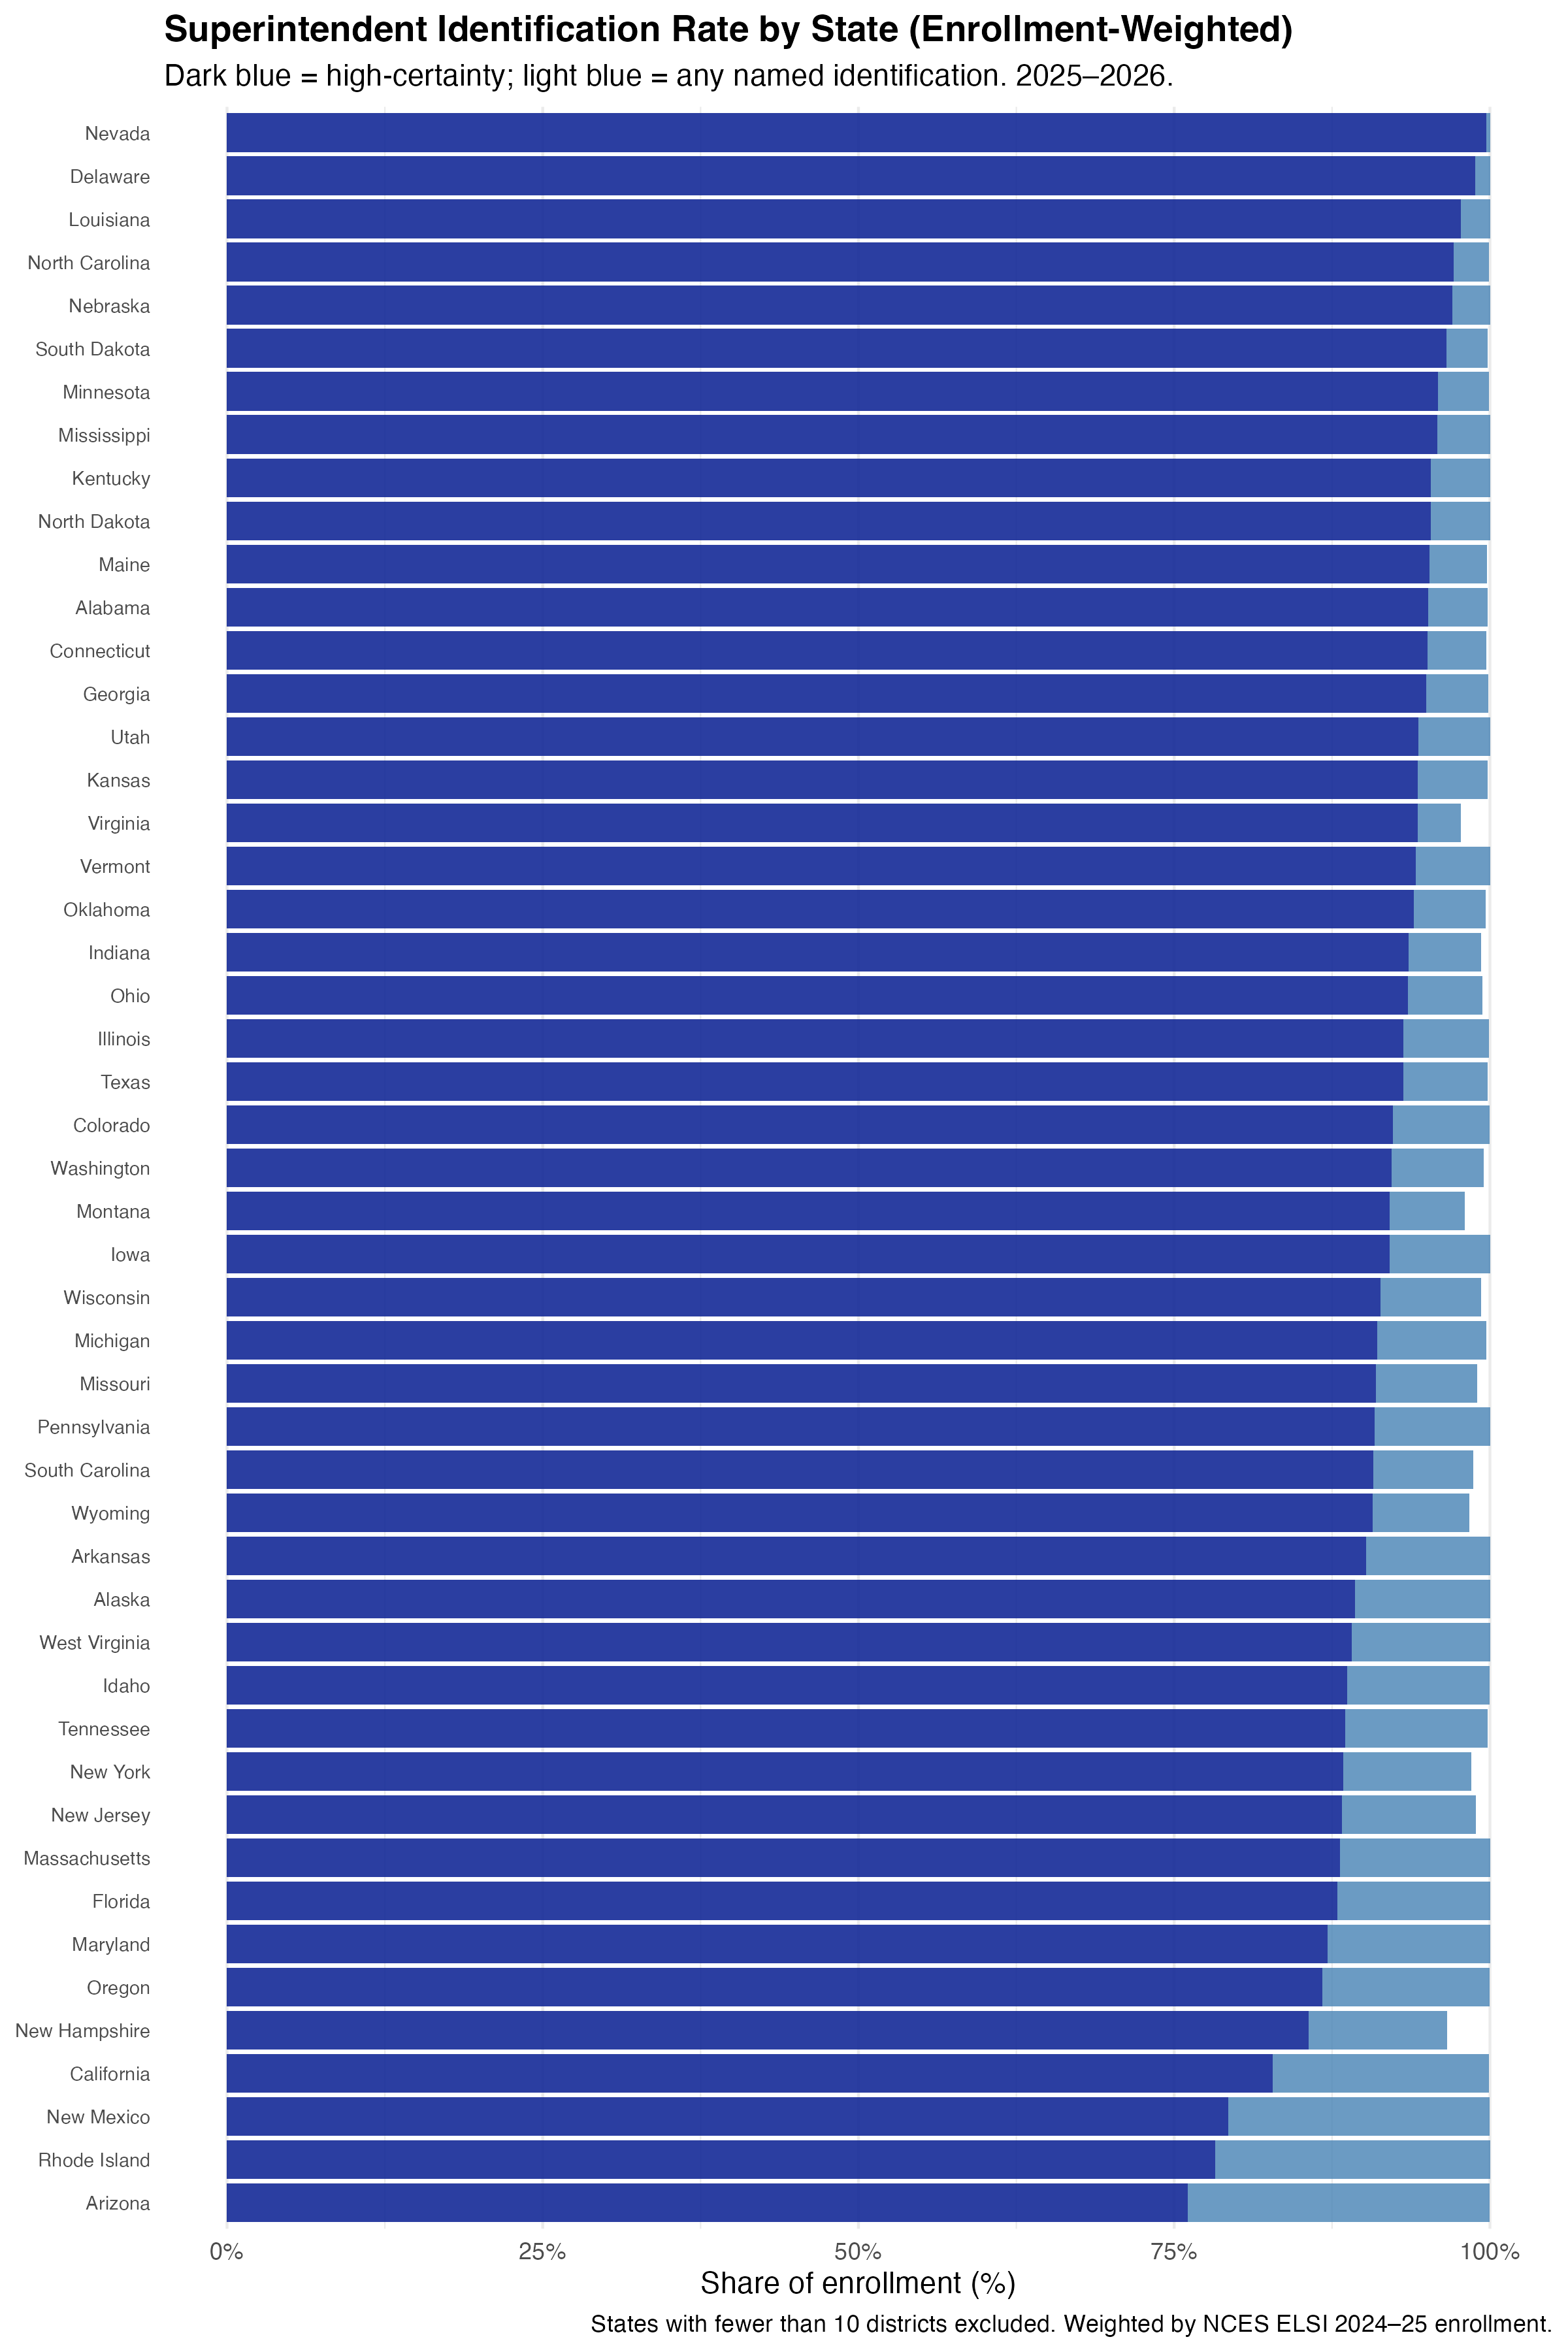
\includegraphics[width=0.78\textwidth, height=0.78\textheight, keepaspectratio]{../figures/fig1_coverage_by_state.png}
    \caption*{\footnotesize Notes: Dark blue bars show the share of enrollment in districts with a high-certainty identification; light blue bars show the share in districts with any named identification (high, medium, or low certainty combined). States with fewer than 10 districts are excluded. Enrollment figures from \citet{nces_ccd}.}
\end{figure}

\section*{Tables}

\begingroup\fontsize{9}{11}\selectfont

\begin{longtable}[t]{lrrrr}
\caption{\label{tab:combined}District Identification Rates by State, 2025--2026}\\
\toprule
State & Total districts & Named (\%) & High cert. (\%) & Enroll. covered (\%)\\
\midrule
\endfirsthead
\caption[]{District Identification Rates by State, 2025--2026 \textit{(continued)}}\\
\toprule
State & Total districts & Named (\%) & High cert. (\%) & Enroll. covered (\%)\\
\midrule
\endhead

\endfoot
\bottomrule
\endlastfoot
Alabama & 139 & 99.3 & 88.5 & 99.8\\
Alaska & 52 & 100.0 & 73.1 & 100.0\\
Arizona & 217 & 96.3 & 86.6 & 100.0\\
Arkansas & 233 & 100.0 & 88.4 & 100.0\\
California & 988 & 99.5 & 88.8 & 99.9\\
\addlinespace
Colorado & 178 & 99.4 & 93.8 & 100.0\\
Connecticut & 168 & 97.6 & 91.7 & 99.7\\
Delaware & 19 & 100.0 & 94.7 & 100.0\\
District Of Columbia & 1 & 100.0 & 0.0 & 100.0\\
Florida & 67 & 100.0 & 95.5 & 100.0\\
\addlinespace
Georgia & 180 & 99.4 & 92.2 & 99.9\\
Guam & 1 & 100.0 & 0.0 & 100.0\\
Hawaii & 1 & 100.0 & 100.0 & 100.0\\
Idaho & 115 & 98.3 & 85.2 & 100.0\\
Illinois & 853 & 99.6 & 91.3 & 99.9\\
\addlinespace
Indiana & 291 & 98.6 & 91.4 & 99.3\\
Iowa & 325 & 100.0 & 92.3 & 100.0\\
Kansas & 286 & 99.3 & 90.2 & 99.8\\
Kentucky & 171 & 100.0 & 91.8 & 100.0\\
Louisiana & 69 & 100.0 & 92.8 & 100.0\\
\addlinespace
Maine & 192 & 97.9 & 88.0 & 99.8\\
Maryland & 24 & 100.0 & 91.7 & 100.0\\
Massachusetts & 323 & 100.0 & 89.5 & 100.0\\
Michigan & 536 & 97.9 & 88.8 & 99.7\\
Minnesota & 327 & 99.4 & 93.3 & 99.9\\
\addlinespace
Mississippi & 138 & 100.0 & 92.0 & 100.0\\
Missouri & 518 & 98.3 & 87.3 & 99.0\\
Montana & 390 & 92.6 & 68.7 & 98.0\\
Nebraska & 243 & 100.0 & 91.4 & 100.0\\
Nevada & 17 & 100.0 & 88.2 & 100.0\\
\addlinespace
New Hampshire & 165 & 96.4 & 81.2 & 96.6\\
New Jersey & 559 & 98.9 & 85.2 & 98.9\\
New Mexico & 89 & 98.9 & 78.7 & 100.0\\
New York & 718 & 99.9 & 92.1 & 98.5\\
North Carolina & 122 & 95.1 & 86.9 & 99.9\\
\addlinespace
North Dakota & 166 & 100.0 & 88.6 & 100.0\\
Northern Marianas & 1 & 100.0 & 0.0 & 100.0\\
Ohio & 617 & 98.5 & 89.5 & 99.4\\
Oklahoma & 507 & 98.6 & 89.5 & 99.7\\
Oregon & 171 & 98.2 & 86.5 & 100.0\\
\addlinespace
Pennsylvania & 499 & 100.0 & 90.8 & 100.0\\
Puerto Rico & 1 & 100.0 & 100.0 & 100.0\\
Rhode Island & 36 & 100.0 & 75.0 & 100.0\\
South Carolina & 74 & 95.9 & 83.8 & 98.7\\
South Dakota & 148 & 99.3 & 91.2 & 99.8\\
\addlinespace
Tennessee & 140 & 99.3 & 80.7 & 99.8\\
Texas & 1020 & 98.9 & 88.0 & 99.8\\
U.S. Virgin Islands & 2 & 100.0 & 100.0 & 100.0\\
Utah & 41 & 100.0 & 95.1 & 100.0\\
Vermont & 105 & 100.0 & 94.3 & 100.0\\
\addlinespace
Virginia & 131 & 98.5 & 90.8 & 97.7\\
Washington & 298 & 97.7 & 89.3 & 99.5\\
West Virginia & 55 & 100.0 & 83.6 & 100.0\\
Wisconsin & 420 & 98.6 & 86.0 & 99.3\\
Wyoming & 48 & 95.8 & 87.5 & 98.4\\
\addlinespace
TOTAL & 13195 & 98.8 & 88.5 & 99.6\\
\end{longtable}
\endgroup{}

{\footnotesize Notes: Named (\%) is the share of CCD-listed open regular public school districts with a named superintendent. High cert.\ (\%) is the share with a high-confidence identification (evidence score $\geq$ 5). Enroll.\ covered (\%) is the share of total district enrollment in districts with a named superintendent. Enrollment figures from \citet{nces_ccd}.}

\bigskip

\begingroup\fontsize{9}{11}\selectfont

\begin{longtable}[t]{lrr}
\caption{\label{tab:gender_comparison}Share of male superintendents (\%): comparison to \citet{superintendentlab}}\\
\toprule
State & Our Data (2025--26) & Sup.\ Lab (2024--25)\\
\midrule
\endfirsthead
\caption[]{Share of male superintendents (\%): comparison to \citet{superintendentlab} \textit{(continued)}}\\
\toprule
State & Our Data (2025--26) & Sup.\ Lab (2024--25)\\
\midrule
\endhead

\endfoot
\bottomrule
\endlastfoot
AK & 60.8 & 63.4\\
AL & 72.2 & 77\\
AR & 74.2 & 73.8\\
AZ & 58.9 & 58.6\\
CA & 54.8 & 57.2\\
\addlinespace
CO & 64.4 & 67.3\\
CT & 63.4 & 62.9\\
DC & 100 & --\\
DE & 72.2 & 81.2\\
FL & 71.2 & 71.1\\
\addlinespace
GA & 61.1 & 71.4\\
HI & 100 & --\\
IA & 84 & 86.9\\
ID & 67.9 & 73.9\\
IL & 67.7 & 71.8\\
\addlinespace
IN & 75.2 & 79.3\\
KS & 74 & 80.5\\
KY & 79.2 & 81\\
LA & 68.2 & 71.8\\
MA & 61.6 & 59\\
\addlinespace
MD & 52.4 & 59\\
ME & 59.6 & 64.1\\
MI & 72.8 & 75.3\\
MN & 76.8 & 81.8\\
MO & 71.2 & 73\\
\addlinespace
MS & 73.7 & 75.8\\
MT & 59.2 & 67.1\\
NC & 72.8 & 74.5\\
ND & 75.2 & 78.8\\
NE & 85.6 & 85.8\\
\addlinespace
NH & 52.8 & 62.5\\
NJ & 62.2 & 65.6\\
NM & 61.9 & 61.9\\
NV & 93.3 & 78.4\\
NY & 67.9 & 71\\
\addlinespace
OH & 80.9 & 83.1\\
OK & 75.3 & 78.7\\
OR & 63.6 & 67.3\\
PA & 76.3 & 75\\
RI & 63.9 & 58.8\\
\addlinespace
SC & 66.7 & 73.6\\
SD & 74.8 & 79.3\\
TN & 65.4 & 71.6\\
TX & 70.5 & 74.6\\
UT & 82.5 & 85.8\\
\addlinespace
VA & 59.8 & 64\\
VT & 51.4 & 54.9\\
WA & 65.2 & 71.9\\
WI & 74.1 & 74.8\\
WV & 58.2 & 63.3\\
\addlinespace
WY & 80.4 & 79.8\\
TOTAL & 69 & 74.1\\*
\end{longtable}
\endgroup{}

{\footnotesize Notes: Gender is predicted from the superintendent's first name using the \textbf{gender} package in R. Our data cover the 2025--26 school year; the right column is from \citet{superintendentlab}, covering 2024--25. The TOTAL row for our data is computed across all 13,037 named districts nationally; the Superintendent Lab figure (74.1\%) is as reported by \citet{superintendentlab} and may reflect a different sample or weighting than the state-level values shown. ``--'' indicates states not covered by the Superintendent Lab data.}

\newpage
\printbibliography

\end{document}
